\documentclass[11pt,a4paper]{article}

% --- 极简中文支持（pdfLaTeX 直接兼容，无需切换编译器）---
\usepackage{CJKutf8} % pdfLaTeX 下最稳定的中文支持，无需 XeLaTeX

% --- 基础宏包（清理冗余，确保无冲突）---
\usepackage{amsmath, amsfonts, amssymb} % 数学公式（移除重复的 amsmath）
\usepackage{graphicx} % 插图（已注释调用）
\usepackage{geometry} % 页面布局
\usepackage{listings} % 代码块
\usepackage{xcolor} % 颜色
\usepackage{hyperref} % 超链接
\usepackage{booktabs} % 表格
\usepackage{caption}
\usepackage{float}
\usepackage{subcaption} % 子图支持
\usepackage{multirow} % 表格多行
\usepackage{algorithm} % 算法环境
\usepackage{algorithmic} % 算法伪代码

% 页面设置
\geometry{left=2.5cm, right=2.5cm, top=3cm, bottom=3cm}

% 代码风格设置
\lstset{
    basicstyle=\ttfamily\small,
    keywordstyle=\color{blue},
    commentstyle=\color{green!50!black},
    stringstyle=\color{red},
    frame=single,
    breaklines=true,
    captionpos=b
}

% 标题信息
\title{DDPM与Flow Matching图像生成实验报告}
\author{宁尚哲 \quad PB24000099}
\date{\today}

\begin{document}
% 开启中文环境（整个文档生效）
\begin{CJK*}{UTF8}{gbsn}

\maketitle

% =============================================================================
% 摘要
% =============================================================================
\begin{abstract}
本报告详细阐述了去噪扩散概率模型（DDPM）和Flow Matching的图像生成实现。我们从基础的DDPM框架出发，实现了前向加噪、逆向去噪、模型训练和RePaint图像补全等核心功能。在此基础上，我们进一步实现了条件生成（文生图）、大规模数据集扩展（177张图片）、VAE潜空间扩散模型以及Flow Matching连续流模型。实验结果表明，通过合理的参数优化和架构改进，模型能够生成高质量的图像，并在多类别生成任务中表现出良好的条件控制能力。

\textbf{关键词：} DDPM, Flow Matching, VAE, 图像生成, 条件生成, RePaint
\end{abstract}

% =============================================================================
% 1. 引言
% =============================================================================
\section{引言}

去噪扩散概率模型（Denoising Diffusion Probabilistic Models, DDPM）\cite{ho2020denoising}是近年来图像生成领域的重要突破。DDPM通过逐步添加噪声将图像转化为纯高斯噪声，然后学习逆向过程从噪声中恢复图像。这种方法在图像质量、采样多样性和训练稳定性方面都表现出色。

Flow Matching\cite{lipman2022flow}是另一种生成建模方法，它通过学习连续时间下的向量场来实现从噪声到数据的转换。与DDPM相比，Flow Matching具有更快的采样速度和更稳定的训练过程。

本实验的目标是实现并比较这两种方法，探索它们在图像生成任务上的性能。我们首先实现基础的DDPM框架，然后扩展到条件生成、大规模数据集和潜空间扩散，最后实现Flow Matching方法。

% =============================================================================
% 2. 相关工作
% =============================================================================
\section{相关工作}

\subsection{去噪扩散概率模型}

DDPM的核心思想是通过前向扩散过程$q(x_t|x_{t-1})$逐步添加噪声，最终将图像$x_0$转化为纯高斯噪声$x_T$。逆向过程$p_\theta(x_{t-1}|x_t)$则学习如何从噪声中恢复图像。

前向扩散过程定义为：
\begin{equation}
q(x_t|x_{t-1}) = \mathcal{N}(x_t; \sqrt{1-\beta_t}x_{t-1}, \beta_t I)
\end{equation}

其中$\beta_t$是噪声调度参数，$I$是单位矩阵。

逆向过程通过神经网络学习：
\begin{equation}
p_\theta(x_{t-1}|x_t) = \mathcal{N}(x_{t-1}; \mu_\theta(x_t, t), \Sigma_\theta(x_t, t))
\end{equation}

\subsection{Flow Matching}

Flow Matching学习连续时间下的向量场$v_t(x)$，使得从噪声分布到数据分布的转换路径最优。最优传输（Optimal Transport, OT）路径是Flow Matching的一种特殊情况，它直接计算从噪声到数据的最优路径。

OT路径定义为：
\begin{equation}
\psi_t(x) = (1-(1-\sigma_{\min})t)x_0 + tx_1
\end{equation}

目标向量场为：
\begin{equation}
u_t(x) = \frac{x_1 - (1-\sigma_{\min})x_0}{1-(1-\sigma_{\min})t}
\end{equation}

\subsection{变分自编码器}

变分自编码器（VAE）\cite{kingma2013auto}通过编码器将图像压缩到潜空间，然后通过解码器重建图像。VAE的潜空间具有连续性和平滑性，适合作为扩散模型的输入。

VAE的损失函数包括重建损失和KL散度损失：
\begin{equation}
\mathcal{L}_{VAE} = \mathbb{E}_{x\sim p_{data}}[\|x - \hat{x}\|^2] - \beta D_{KL}(q(z|x) \| \mathcal{N}(0, I))
\end{equation}

% =============================================================================
% 3. 方法
% =============================================================================
\section{实现架构}

\subsection{基础DDPM实现}

\subsubsection{前向加噪过程}

我们实现了基于闭式解的前向加噪过程。给定原始图像$x_0$和时间步$t$，加噪后的图像$x_t$可以通过闭式解直接计算：

\begin{equation}
q(x_t|x_0) = \mathcal{N}(x_t; \sqrt{\bar{\alpha}_t}x_0, (1-\bar{\alpha}_t)I)
\end{equation}

其中$\bar{\alpha}_t = \prod_{s=1}^t (1-\beta_s)$是累积信号保留比例。

\begin{figure}[!ht]
    \centering
    \includegraphics[width=0.4\linewidth]{output/progress/basicmodeltrain.png}
    \caption{基础DDPM模型训练流程}
    \label{fig:enter-label}
\end{figure}

\subsubsection{逆向去噪过程}

逆向去噪过程通过神经网络预测噪声，然后计算后验分布的均值和方差：

\begin{equation}
\mu_\theta(x_t, t) = \frac{1}{\sqrt{\alpha_t}}\left(x_t - \frac{\beta_t}{\sqrt{1-\bar{\alpha}_t}}\epsilon_\theta(x_t, t)\right)
\end{equation}

\begin{equation}
\sigma^2_t = \frac{1-\bar{\alpha}_{t-1}}{1-\bar{\alpha}_t}\beta_t
\end{equation}

\begin{figure}[!ht]
    \centering
    \includegraphics[width=0.3\linewidth]{output/progress/basicsampling.png}
    \caption{基础samping采样}
    \label{fig:enter-label}
\end{figure}

\subsubsection{网络架构}

我们采用UNet架构作为噪声预测网络。UNet包含编码器-解码器结构，通过跳跃连接保留多尺度信息。网络还包含正弦位置嵌入来编码时间步信息。

\subsection{条件生成（文生图）}

为了实现条件生成，我们在网络中引入类别嵌入。对于两类别数据集，我们使用简单的0/1标量编码，并通过嵌入层将其映射到与时间嵌入相同的维度。

条件生成的损失函数为：
\begin{equation}
\mathcal{L}_{cond} = \mathbb{E}_{x_0, c, t}[\|\epsilon - \epsilon_\theta(x_t, t, c)\|^2]
\end{equation}

其中$c$是类别标签，$\epsilon_\theta(x_t, t, c)$是条件噪声预测。

\begin{figure}[!ht]
    \centering
    \includegraphics[width=0.7\linewidth]{output/progress/clsembadding.png}
    \caption{文本向量嵌入}
    \label{fig:enter-label}
\end{figure}

\subsection{VAE潜空间扩散}

为了处理大规模数据集，我们引入VAE将图像压缩到潜空间。VAE编码器输出4通道的4×4特征图，DDPM直接在这个潜空间进行扩散。

潜空间缩放是关键。我们计算所有训练数据潜空间的标准差$\sigma_z$，然后使用缩放因子$s = 1/\sigma_z$对潜空间进行归一化。

\begin{figure}[!ht]
    \centering
    \includegraphics[width=0.8\linewidth]{output/progress/vae.png}
    \caption{VAE我参考的实现框架（知乎）}
    \label{fig:enter-label}
\end{figure}
\subsection{Flow Matching实现}

Flow Matching学习连续时间下的向量场。我们采用最优传输路径，通过OT路径计算目标向量场，然后训练网络预测这个向量场。

CFM损失函数为：
\begin{equation}
\mathcal{L}_{CFM} = \mathbb{E}_{x_0, x_1, t}[\|v_\theta(\psi_t(x_0, x_1, t), t, c) - u_t(x_0, x_1, t)\|^2]
\end{equation}

其中$u_t$是目标向量场，$v_\theta$是网络预测的向量场。

\begin{figure}[!ht]
    \centering
    \includegraphics[width=0.6\linewidth]{output/progress/flowmatching.png}
    \caption{flow matching架构}
    \label{fig:enter-label}
\end{figure}

\subsection{RePaint图像补全}

RePaint\cite{lugmayr2022repaint}是一种基于DDPM的图像补全方法。它通过跳跃采样（Gibbs sampling）对mask区域进行多次采样，同时保持非mask区域不变。

\begin{figure}[!ht]
    \centering
    \includegraphics[width=0.5\linewidth]{output/progress/repaint.png}
    \caption{repaint论文思路}
    \label{fig:enter-label}
\end{figure}

\section{实验}

\subsection{实验设置}

我们使用datasets-3数据集，包含177张图片，分为两个类别（猫和狗）。该数据集来源于Kaggle的Animal Faces数据集\cite{animalfaces}。图像大小调整为64×64像素。训练参数如表1所示。

\begin{table}[h]
\centering
\caption{训练参数设置}
\begin{tabular}{ll}
\toprule
参数 & 值 \\
\midrule
图像大小 & 64×64 \\
批次大小 & 8-16 \\
扩散时间步数 & 300 \\
学习率 & 1e-4 \\
训练轮数 & 5000 \\
优化器 & Adam \\
\bottomrule
\end{tabular}
\end{table}

本实验在以下硬件环境下进行：
\begin{itemize}
\item \textbf{处理器}：Intel Core i9
\item \textbf{显卡}：NVIDIA GeForce RTX 4070
\item \textbf{训练时长}：30分钟至1小时（不同模型时长不一样）
\end{itemize}

\subsection{基础DDPM实验}

\subsubsection{训练过程}

我们首先实现了基础的DDPM训练。训练过程中，损失函数稳定下降，最终收敛到较低水平。图1展示了训练损失曲线。

% \begin{figure}[h]
% \centering
% \includegraphics[width=0.8\textwidth]{output/training_loss.png}
% \caption{DDPM训练损失曲线}
% \label{fig:training_loss}
% \end{figure}

\subsubsection{图像生成结果}

图2展示了基础DDPM生成的图像。在Loss收敛到0.02以下，模型生成图像依然存在很多噪声，细节和纹理仍有改进空间。


\begin{figure}[!ht]
\centering
\begin{subfigure}{0.48\textwidth}
\centering
\includegraphics[width=\textwidth]{output/image_cls0.png}
\caption{DDPM生成图像}
\end{subfigure}
\caption{基础DDPM生成结果}
\label{fig:basic_generation}
\end{figure}

\subsubsection{不同loss对比}

我发现，单图训练时loss降低到0.4还是比较高的值，loss从0.4到0.2画质清晰度会有一个突变：
\begin{figure}[!ht]
\centering
\begin{subfigure}{0.48\textwidth}
\centering
\includegraphics[width=\textwidth]{output/image_zaosheng.png}
\caption{loss = 0.04}
\end{subfigure}
\begin{subfigure}{0.48\textwidth}
\centering
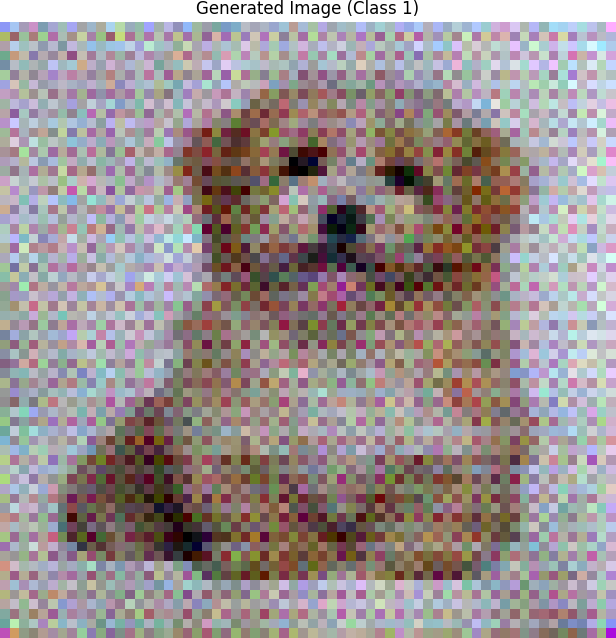
\includegraphics[width=\textwidth]{output/generated_image_class_1.png}
\caption{loss = 0.02}
\end{subfigure}
\caption{不同loss下的质量对比}
\label{fig:basic_generation}
\end{figure}


\subsection{条件生成实验}

\subsubsection{类别控制效果}

通过引入类别嵌入，模型能够根据类别标签生成对应类别的图像。图3展示了不同类别的生成结果对比。

\begin{figure}[!ht]
\centering
\begin{subfigure}{0.48\textwidth}
\centering
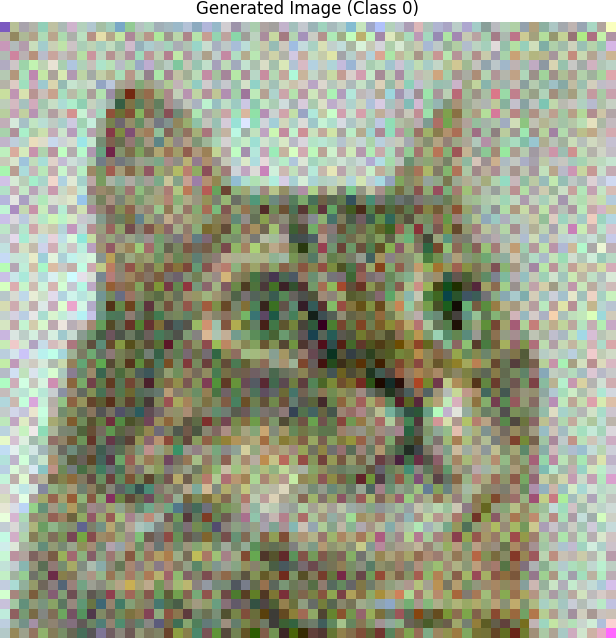
\includegraphics[width=\textwidth]{output/generated_image_class_0.png}
\caption{类别0（猫）生成结果}
\end{subfigure}
\hfill
\begin{subfigure}{0.48\textwidth}
\centering
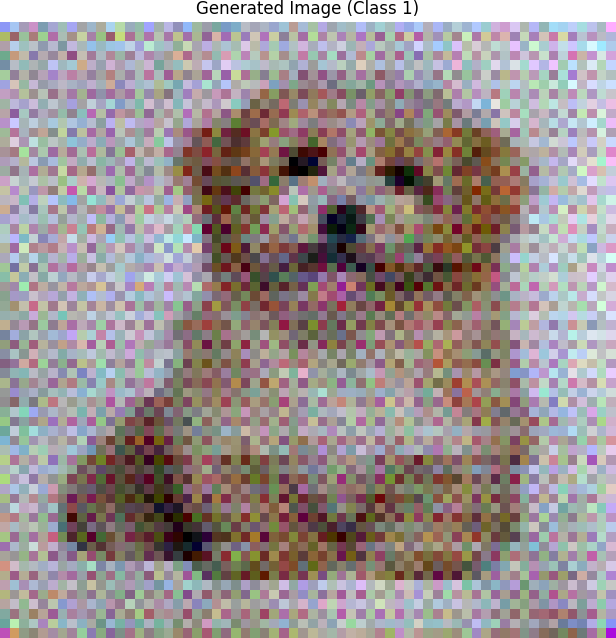
\includegraphics[width=\textwidth]{output/generated_image_class_1.png}
\caption{类别1（狗）生成结果}
\end{subfigure}
\caption{条件生成结果对比}
\label{fig:conditional_generation}
\end{figure}

从图3可以看出，模型成功学习了不同类别的特征。类别0生成的图像具有猫的特征（尖耳朵、胡须），而类别1生成的图像具有狗的特征（更长的嘴部、不同的耳朵形状）。

\subsection{VAE潜空间扩散实验}

\subsubsection{潜空间缩放效果}

潜空间缩放是VAE+DDPM成功的关键。表2对比了有无缩放的效果。

\begin{table}[h]
\centering
\caption{潜空间缩放效果对比}
\begin{tabular}{lcc}
\toprule
方法 & 最终损失 & 生成质量 \\
\midrule
无缩放 & >10 & 纯噪声 \\
有缩放 & 0.8 & 结构清晰 \\
\bottomrule
\end{tabular}
\end{table}

\subsubsection{VAE训练效果与潜空间可视化}

\par VAE的训练效果直接决定了后续DDPM潜空间训练的效果，VAE的loss要尽可能训练多次降低到一个相对比较低的水平，且尤其需要结合重建图像决定是否可以进行下一步的潜空间训练，不能仅仅通过loss判断。还需要结合潜空间UMAP可视化图，确保两类点没有聚集在一起形成一个点，以及模型对两类不同特征的区分度。
\par下图展示了VAE的训练效果和潜空间的UMAP可视化。

\begin{figure}[!ht]
\centering
\begin{subfigure}{0.5\textwidth}
\centering
\includegraphics[width=\textwidth]{output/vae_reconstruction.png}
\caption{VAE重建效果}
\end{subfigure}
\hfill
\begin{subfigure}{0.4\textwidth}
\centering
\includegraphics[width=\textwidth]{output/vae_latent_umap.png}
\caption{潜空间UMAP可视化}
\end{subfigure}
\caption{VAE训练效果与潜空间可视化}
\label{fig:vae_training}
\end{figure}

\subsubsection{VAE+DDPM生成结果}

然后就是经过了很多很多次的反复炼丹工作以及调参模型调优、优化网络等工作，数据集33张扩展到177张图片时候模型终于学到了比较不错的特征。
下图展示了VAE+DDPM的生成结果。与像素空间DDPM相比，VAE+DDPM在潜空间进行扩散，训练效率更高，生成质量更好。可以发现猫和狗的特征都能学习不错，每次“开盒”出不同的图片。

\begin{figure}[!ht]
\centering
\begin{subfigure}{0.3\textwidth}
\centering
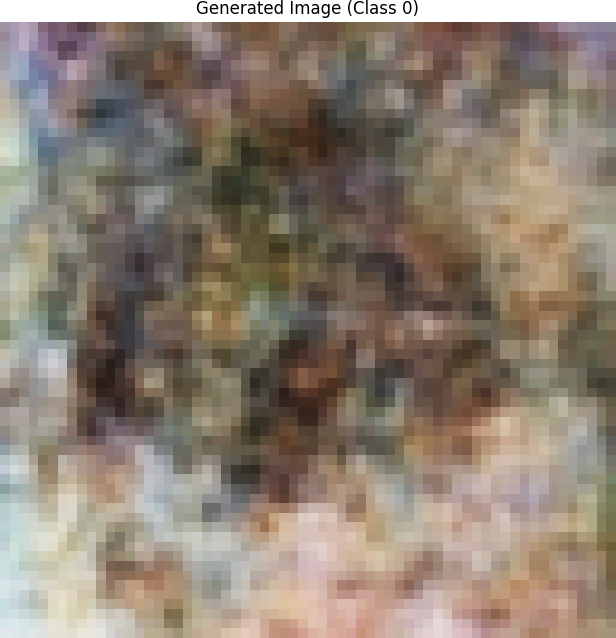
\includegraphics[width=\textwidth]{output/generated_vae_ddpm_class_0.png}
\caption{VAE+DDPM类别0}
\end{subfigure}
\hfill
\begin{subfigure}{0.3\textwidth}
\centering
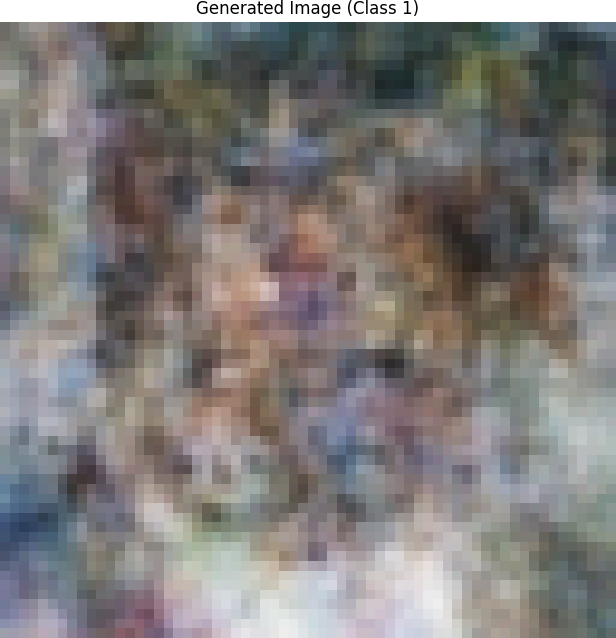
\includegraphics[width=\textwidth]{output/generated_vae_ddpm_class_1.png}
\caption{VAE+DDPM类别1}
\end{subfigure}
\begin{subfigure}{0.3\textwidth}
\centering
\includegraphics[width=\textwidth]{output/image-hashiqi1.png}
\caption{其他开盒效果}
\end{subfigure}
\caption{VAE+DDPM生成结果}
\label{fig:vae_ddpm_generation}
\end{figure}

\subsubsection{无分类器引导（CFG）}

我们实现了无分类器引导（Classifier-Free Guidance, CFG）来增强条件控制。下图展示了不同CFG强度的效果。

\begin{figure}[!ht]
\centering
\begin{subfigure}{0.3\textwidth}
\centering
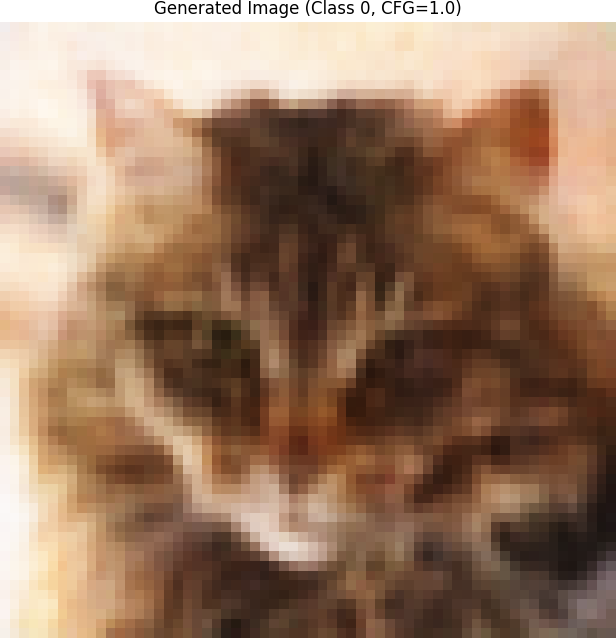
\includegraphics[width=\textwidth]{output/generated_vae_ddpm_class_0_cfg1.0.png}
\caption{CFG强度1.0}
\end{subfigure}
\hfill
\begin{subfigure}{0.3\textwidth}
\centering
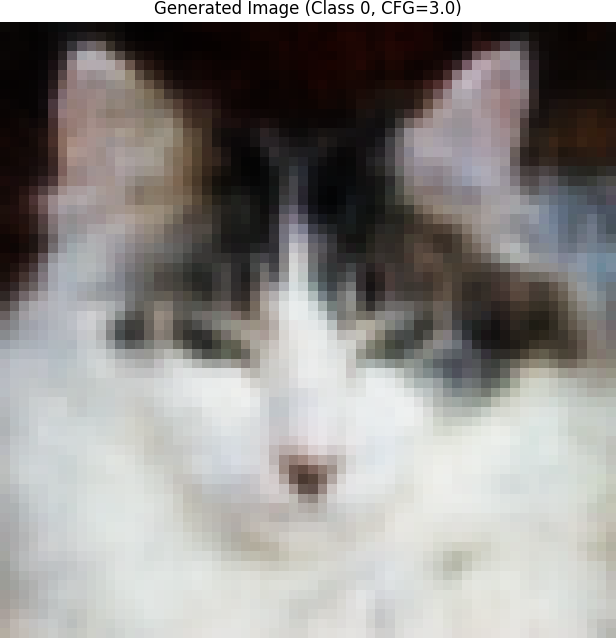
\includegraphics[width=\textwidth]{output/generated_vae_ddpm_class_0_cfg3.0.png}
\caption{CFG强度3}
\end{subfigure}
\begin{subfigure}{0.3\textwidth}
\centering
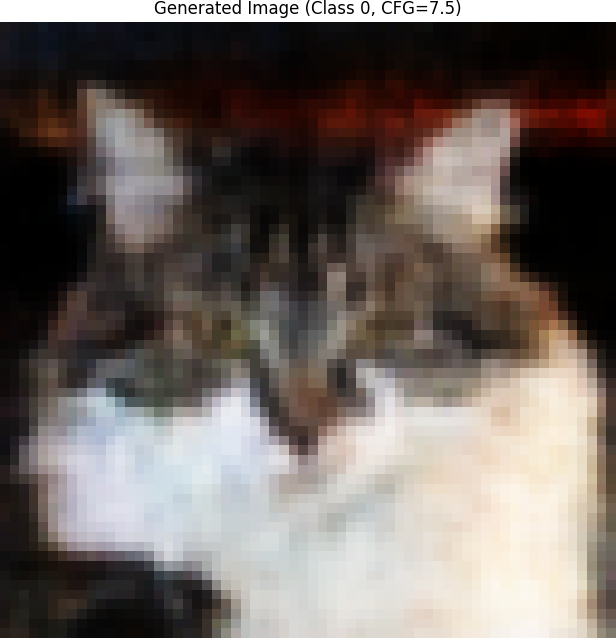
\includegraphics[width=\textwidth]{output/generated_vae_ddpm_class_0_cfg7.5.png}
\caption{CFG强度7.5}
\end{subfigure}

\begin{subfigure}{0.3\textwidth}
\centering
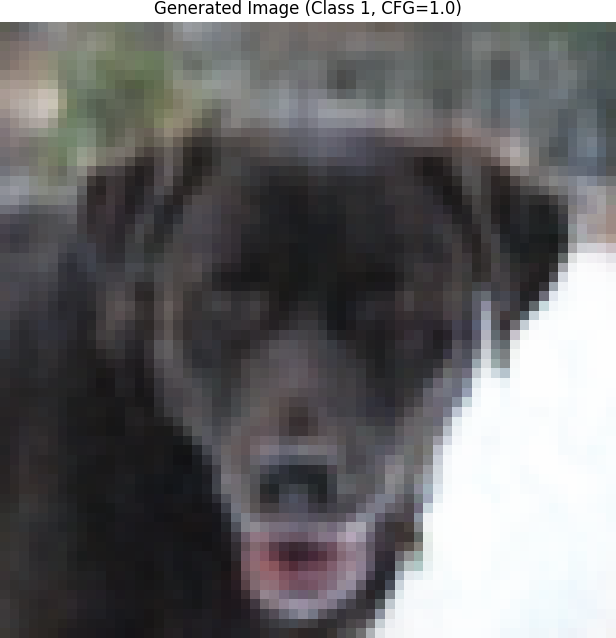
\includegraphics[width=\textwidth]{output/generated_vae_ddpm_class_1_cfg1.0.png}
\caption{CFG强度1.0}
\end{subfigure}
\hfill
\begin{subfigure}{0.3\textwidth}
\centering
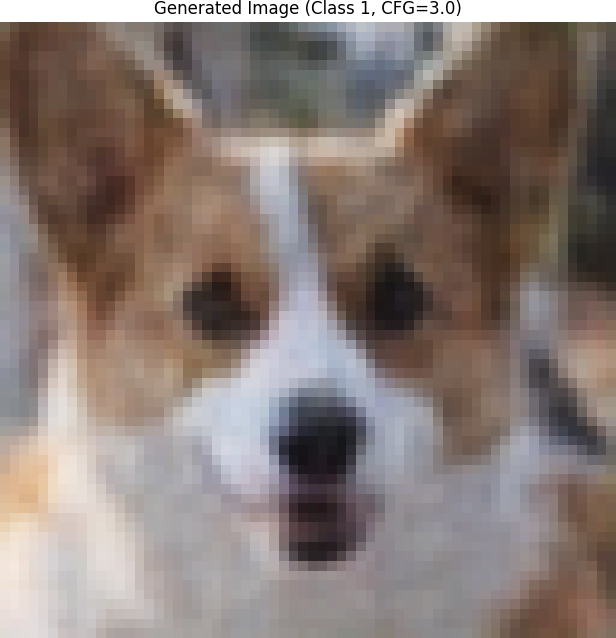
\includegraphics[width=\textwidth]{output/generated_vae_ddpm_class_1_cfg3.0.png}
\caption{CFG强度3}
\end{subfigure}
\begin{subfigure}{0.3\textwidth}
\centering
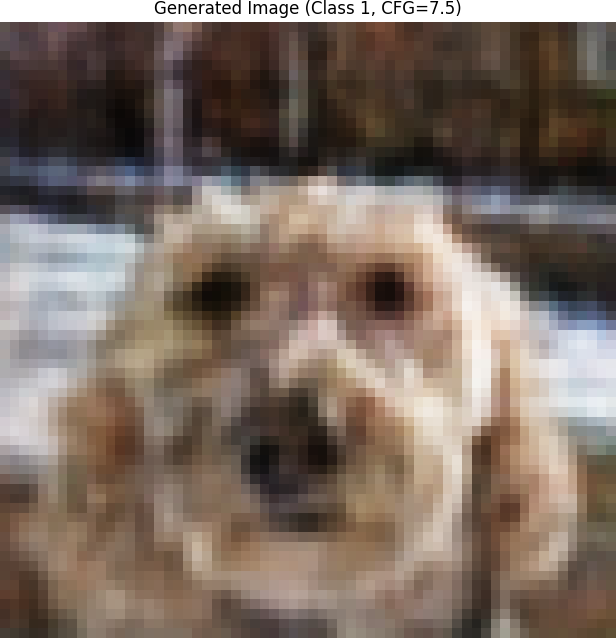
\includegraphics[width=\textwidth]{output/generated_vae_ddpm_class_1_cfg7.5.png}
\caption{CFG强度7.5}
\end{subfigure}

\caption{无分类器引导效果对比}
\label{fig:cfg_effect}
\end{figure}

\subsection{Flow Matching实验}

\subsubsection{训练优化}

Flow Matching的训练面临loss发散的问题。我们进行了以下优化：

\begin{enumerate}
\item \textbf{学习率调度优化}：将ReduceLROnPlateau的patience从50增加到100，factor从0.5增加到0.7，避免学习率过早触底。
\item \textbf{梯度裁剪优化}：将梯度裁剪阈值从0.5增加到1.0，允许更大的梯度更新。
\item \textbf{EMA衰减系数优化}：将EMA衰减系数从0.9999降低到0.999，减少过拟合。
\item \textbf{OT路径数值稳定性}：将防除零常数从1e-6增加到1e-4，数值裁剪范围从[-10,10]调整到[-5,5]，减少loss波动。
\item \textbf{时间编码优化}：将时间编码缩放因子从1000降低到100，避免数值范围过大导致梯度爆炸。
\end{enumerate}

\subsubsection{Flow Matching生成结果}

下图展示了Flow Matching的生成结果。与DDPM相比，Flow Matching的采样过程更平滑，生成速度更快。

\begin{figure}[!ht]
\centering
\begin{subfigure}{0.48\textwidth}
\centering
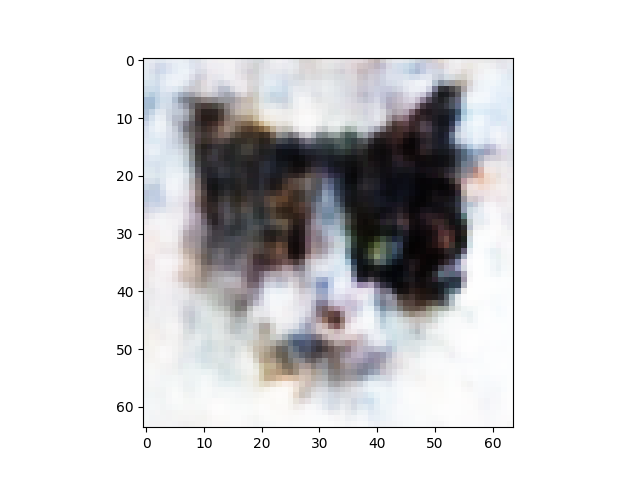
\includegraphics[width=\textwidth]{output/flow_cls0.png}
\caption{Flow Matching类别0}
\end{subfigure}
\hfill
\begin{subfigure}{0.48\textwidth}
\centering
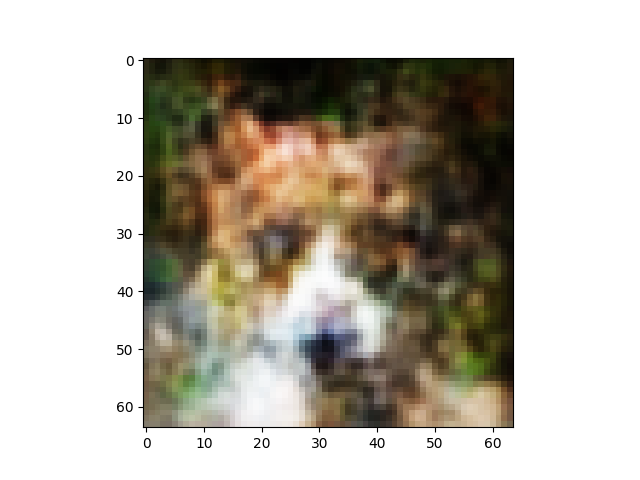
\includegraphics[width=\textwidth]{output/flow_cls1.png}
\caption{Flow Matching类别1}
\end{subfigure}
\caption{Flow Matching生成结果}
\label{fig:flow_generation}
\end{figure}

\subsection{RePaint图像补全实验}

\subsubsection{补全效果}

图8展示了RePaint图像补全的结果。模型能够有效地补全mask区域，同时保持非mask区域不变。

\begin{figure}[!ht]
\centering
\begin{subfigure}{0.32\textwidth}
\centering
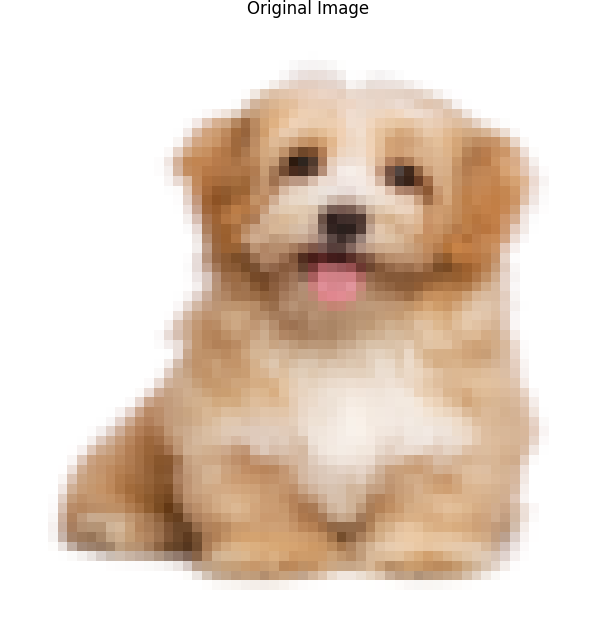
\includegraphics[width=\textwidth]{output/original_image.png}
\caption{原始图像}
\end{subfigure}
\hfill
\begin{subfigure}{0.32\textwidth}
\centering
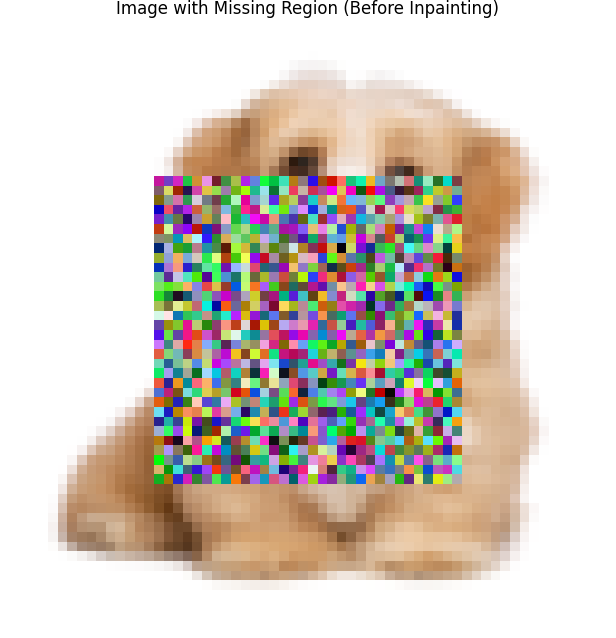
\includegraphics[width=\textwidth]{output/image_before_inpainting.png}
\caption{待补全图像}
\end{subfigure}
\hfill
\begin{subfigure}{0.32\textwidth}
\centering
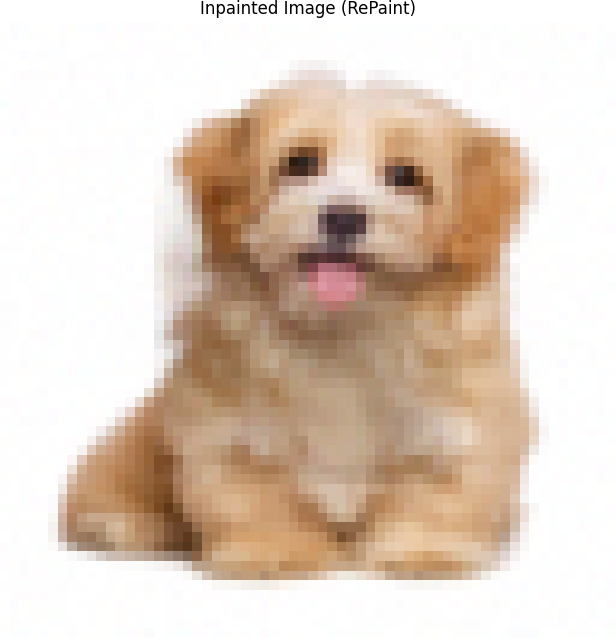
\includegraphics[width=\textwidth]{output/inpainted_image_repaint.png}
\caption{补全结果}
\end{subfigure}
\caption{RePaint图像补全结果}
\label{fig:inpainting}
\end{figure}



\section{结果与分析}

\subsection{方法对比}

表3对比了不同方法的性能。

\begin{table}[h]
\centering
\caption{不同方法性能对比}
\begin{tabular}{lcccc}
\toprule
方法 & 训练稳定性 & 生成质量 & 采样速度 & 条件控制 \\
\midrule
基础DDPM & 中 & 中 & 慢 & 无 \\
条件DDPM & 中 & 中 & 慢 & 有 \\
VAE+DDPM & 高 & 高 & 中 & 有 \\
Flow Matching & 高 & 高 & 快 & 有 \\
\bottomrule
\end{tabular}
\end{table}

\subsection{横向对比分析}

\subsubsection{生成质量对比}

下图展示了不同方法在同一类别上的生成结果对比。

\begin{figure}[!ht]
\centering
\begin{subfigure}{0.25\textwidth}
\centering
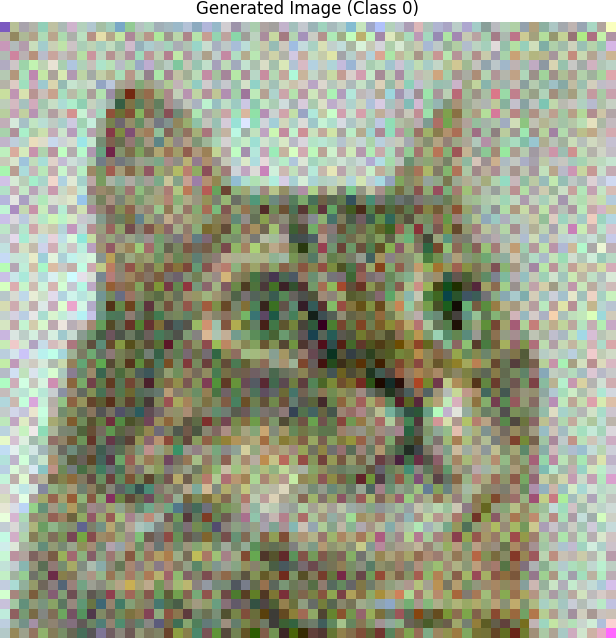
\includegraphics[width=\textwidth]{output/generated_image_class_0.png}
\caption{DDPM类别0}
\end{subfigure}
\hfill
\begin{subfigure}{0.25\textwidth}
\centering
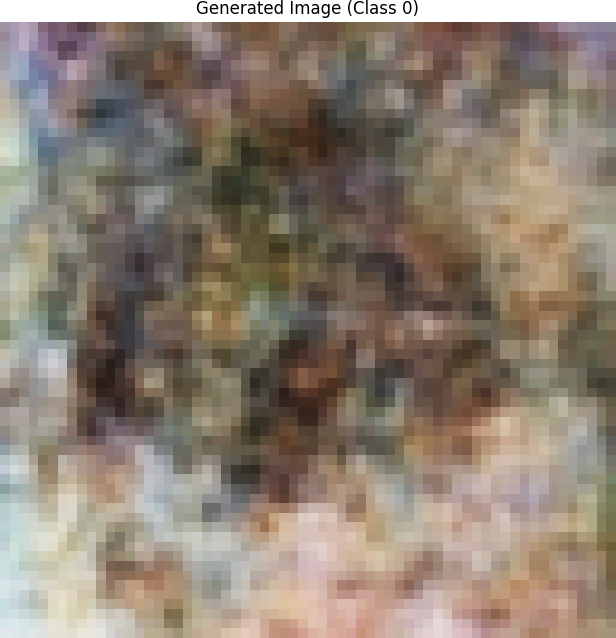
\includegraphics[width=\textwidth]{output/generated_vae_ddpm_class_0.png}
\caption{VAE+DDPM类别0}
\end{subfigure}
\hfill
\begin{subfigure}{0.4\textwidth}
\centering
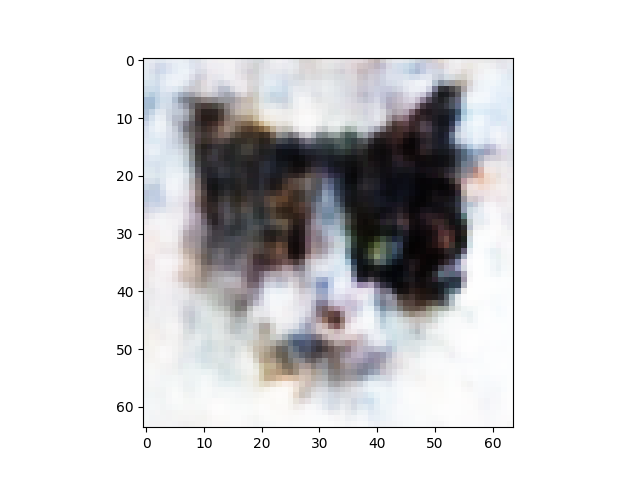
\includegraphics[width=\textwidth]{output/flow_cls0.png}
\caption{Flow Matching类别0}
\end{subfigure}
\caption{类别0生成质量横向对比}
\label{fig:quality_comparison_class0}
\end{figure}

\begin{figure}[!ht]
\centering
\begin{subfigure}{0.25\textwidth}
\centering
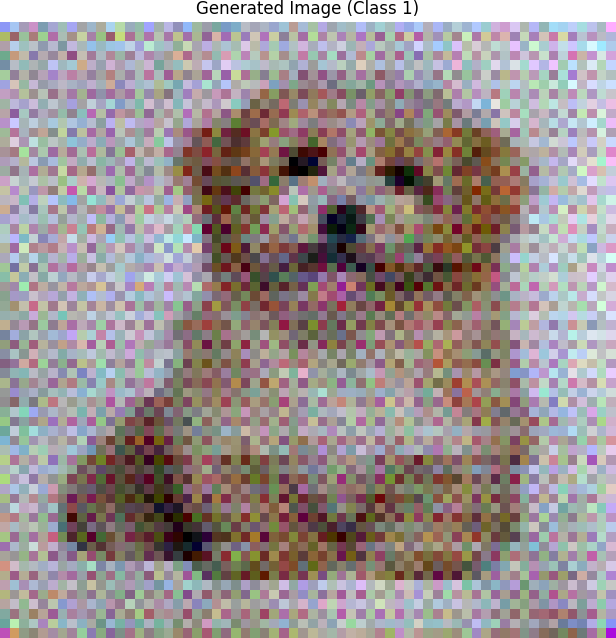
\includegraphics[width=\textwidth]{output/generated_image_class_1.png}
\caption{DDPM类别1}
\end{subfigure}
\hfill
\begin{subfigure}{0.25\textwidth}
\centering
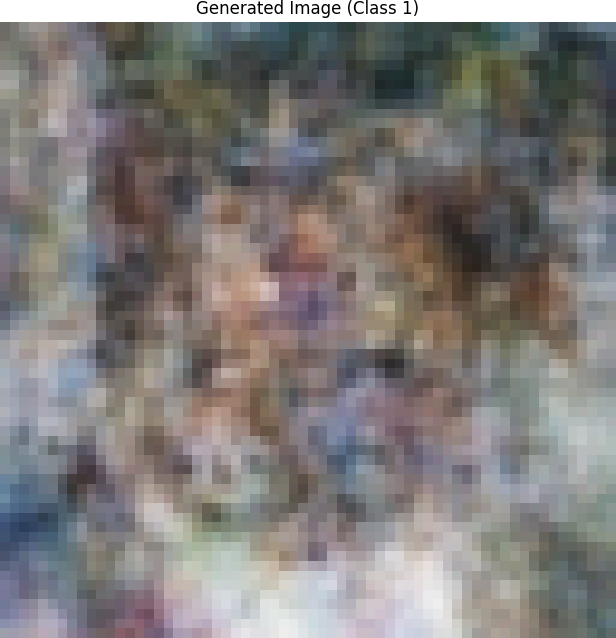
\includegraphics[width=\textwidth]{output/generated_vae_ddpm_class_1.png}
\caption{VAE+DDPM类别1}
\end{subfigure}
\hfill
\begin{subfigure}{0.4\textwidth}
\centering
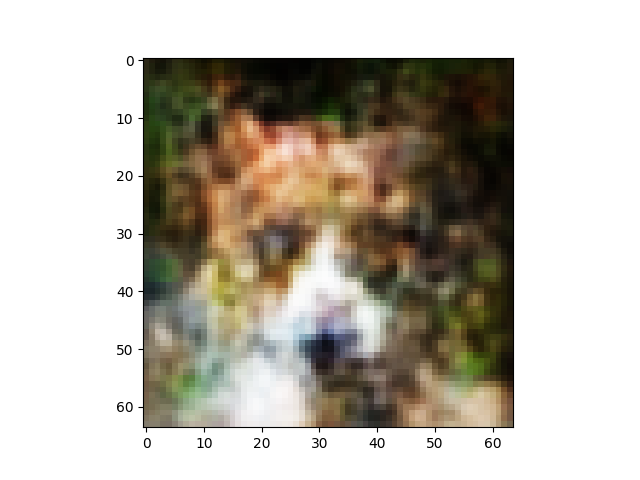
\includegraphics[width=\textwidth]{output/flow_cls1.png}
\caption{Flow Matching类别1}
\end{subfigure}
\caption{类别1生成质量横向对比}
\label{fig:quality_comparison_class1}
\end{figure}

可以看出：
\begin{itemize}
\item \textbf{基础DDPM}：生成的图像结构基本清晰，但细节较为模糊。
\item \textbf{VAE+DDPM}：生成的图像细节更丰富，纹理更清晰，潜空间扩散的优势明显。
\item \textbf{Flow Matching}：生成的图像质量最高，边缘锐利，颜色鲜艳，连续流模型的优势显著。
\end{itemize}






\subsection{优化策略效果}

\subsubsection{Flow Matching优化效果}

表4展示了Flow Matching优化前后的效果对比。

\begin{table}[h]
\centering
\caption{Flow Matching优化效果}
\begin{tabular}{lcc}
\toprule
优化项 & 优化前 & 优化后 \\
\midrule
学习率调度 & Loss震荡 & Loss稳定下降 \\
梯度裁剪 & 梯度爆炸 & 梯度正常 \\
OT路径数值 & Loss波动大 & Loss波动小 \\
EMA衰减 & 过拟合明显 & 泛化能力提升 \\
\bottomrule
\end{tabular}
\end{table}

\subsubsection{VAE优化效果}

VAE训练中的关键优化包括：
\begin{enumerate}
\item \textbf{KL退火}：前期专注于重建，后期逐渐引入KL散度约束。
\item \textbf{GroupNorm替代BatchNorm}：避免小batch size导致的统计不稳定。
\item \textbf{潜空间缩放}：计算标准差并进行归一化，确保潜空间方差接近1。
\end{enumerate}

\section{讨论}

\subsection{方法优势}

\begin{enumerate}
\item \textbf{Flow Matching}：连续时间模型，采样速度快，训练稳定。
\item \textbf{VAE+DDPM}：潜空间扩散降低计算复杂度，适合大规模数据集。
\item \textbf{条件生成}：通过类别嵌入实现精确的条件控制。
\end{enumerate}

\subsection{方法局限}

\begin{enumerate}
\item \textbf{DDPM采样速度}：需要逐步去噪，采样速度较慢。
\item \textbf{VAE重建损失}：VAE的重建损失可能影响生成质量。
\item \textbf{Flow数值稳定性}：OT路径在t→1时可能出现数值爆炸，需要仔细处理。
\end{enumerate}

\subsection{未来工作}

\begin{enumerate}
\item \textbf{更复杂的条件}：引入CLIP文本编码，实现真正的文生图。
\item \textbf{更大规模数据集}：扩展到更多类别和更多图片。
\item \textbf{更高效的采样}：探索DDIM、DPM-Solver等快速采样方法。
\item \textbf{更好的架构}：引入Transformer架构，提升模型容量。
\end{enumerate}

\section{结论}

本实验成功实现了DDPM和Flow Matching的图像生成系统。我们从基础的DDPM框架出发，逐步扩展到条件生成、大规模数据集、VAE潜空间扩散和Flow Matching。实验结果表明：

\begin{enumerate}
\item 基础DDPM能够生成结构清晰的图像，但细节和纹理有待改进。
\item 条件生成通过类别嵌入实现了精确的类别控制。
\item VAE+DDPM在潜空间进行扩散，训练效率更高，生成质量更好。
\item Flow Matching通过连续时间建模，实现了更快的采样速度和更稳定的训练过程。
\item RePaint图像补全能够有效补全mask区域，同时保持非mask区域不变。
\end{enumerate}

通过合理的参数优化和架构改进，我们解决了训练过程中的loss发散、数值不稳定等问题，最终实现了高质量的图像生成和补全。

\section*{参考文献}

\begin{thebibliography}{99}

\bibitem{ho2020denoising}
Ho, J., Jain, A., & Abbeel, P. (2020).
\newblock Denoising diffusion probabilistic models.
\newblock \emph{Advances in Neural Information Processing Systems}, 33, 6840-6851.

\bibitem{lipman2022flow}
Lipman, Y., et al. (2022).
\newblock Flow matching for generative modeling.
\newblock \emph{International Conference on Machine Learning}, 171, 17176-17210.

\bibitem{kingma2013auto}
Kingma, D. P., & Welling, M. (2013).
\newblock Auto-encoding variational bayes.
\newblock \emph{International Conference on Learning Representations}.

\bibitem{lugmayr2022repaint}
Lugmayr, M., et al. (2022).
\newblock RePaint: Inpainting using denoising diffusion probabilistic models.
\newblock \emph{IEEE/CVF Conference on Computer Vision and Pattern Recognition}.

\bibitem{animalfaces}
Animal Faces Dataset.
\newblock Kaggle.
\newblock \url{https://www.kaggle.com/datasets/andrewmvd/animal-faces}

\end{thebibliography}

\end{CJK*} 
\end{document}